Plot the frame M coordinates $(3, -2)_M$ Now express the frame M coordinates $(3, -2)_M$ in the frame G, and confirm that this is the same point by plotting it using the frame G.

\begin{solution}
\begin{align*}
    R_{GM} &= \begin{bmatrix}
        \boldsymbol{\hat{i}}_M \boldsymbol{\hat{i}}_G & \boldsymbol{\hat{j}}_M \boldsymbol{\hat{i}}_G \\
        \boldsymbol{\hat{i}}_M \boldsymbol{\hat{j}}_G & \boldsymbol{\hat{j}}_M \boldsymbol{\hat{j}}_G \\
    \end{bmatrix} \\
    &= \begin{bmatrix}
        \frac{1}{2} & -\frac{\sqrt{3}}{2} \\
        \frac{\sqrt{3}}{2} & \frac{1}{2} \\
    \end{bmatrix} \\
    r_G &= R_{GM} r_M \\
    &= \begin{bmatrix}
        \frac{1}{2} & -\frac{\sqrt{3}}{2} \\
        \frac{\sqrt{3}}{2} & \frac{1}{2} \\
    \end{bmatrix} \begin{bmatrix}
        3 \\ -2
    \end{bmatrix} = \begin{bmatrix}
        3.323 \\ 1.598
    \end{bmatrix} \\
    r_G &= 3.323 \boldsymbol{\hat{i}}_G + 1.598 \boldsymbol{\hat{j}}_G
\end{align*}

\begin{center}
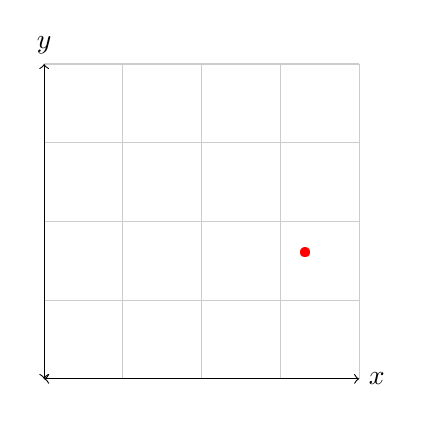
\begin{tikzpicture}
    \draw[thin,gray!40] (0,0) grid (4,4);
    \draw[<->] (0,0)--(4,0) node[right]{$x$};
    \draw[<->] (0,0)--(0,4) node[above]{$y$};
    \node [red] at (3.323, 1.598) {\textbullet};
\end{tikzpicture}
\end{center}
\end{solution}